\section{Systematic Uncertainties}
\label{chap:Systematics}

\subsection{Spectra}
\label{sec:SystematicsSpectra}

Below are the studied sources of systematic uncertainty and their details. For each of the systematics, the analysis was repeated from start to finish for each variation and required either a seperate subwagon or train run. All variations for one systematic contribution are evaluated simultaneously. The five unfolding systematics are also evaluated together. For each bin in each systematic other than unfolding, the mean of the absolute deviations of all variations is found. For unfolding, the maximum of the absolute deviations of all variations is found. In order to suppress unphysical statistical fluctiations, for most contributions, the mean for all bins is then fit with a 0th - 2nd order polynomial. Some contributions remain as binwise, where the binwise uncertainty is not expected to follow a clear pattern. All the uncertainties are then added in quadrature for each bin.

\begin{itemize}
    \item Tracking efficiency: Variations of $\pm 4\%$ are considered.
    
    \item Unfolding
    \begin{itemize}
        \item Regularization: The default number of iterations is 6, and variations of +3/-2 iteration are considered.
        \item Truncation: The raw distribution and the response matrix are truncated at different values. The default minimum accepted jet \pT is 10 GeV. As variations, $\pm 5$ GeV are considered.
        \item Prior: The default prior is Pythia 8, the MC used in the generation of the response. The ratio between the default unfolded solution and the default prior is considered. This ratio is applied as a weight to the response prior to unfolding.
        \item Binning: Four bin variations to the measured input are considered. For a list of the binning, see appendix \ref{sec:appendixSysBinVar}.
        \item Unfolding method: Bayesian is used by default with SVD as a variation. The difference between the bayesian and the SVD method is primarily used in order to account for the discrepancy seen between the two methods in the region where the triggers swap.
    \end{itemize}

    \item EMCAL seed thresholds:
    \begin{itemize}
        \item Default: Seed threshold = 300 MeV, cell threshold = 100 MeV
        \item Low: Seed threshold = 275 MeV, cell threshold = 75 MeV
        \item High: Seed threshold = 350 MeV, cell threshold = 100 MeV
    \end{itemize}
    
    \item Clusterizer algorithm: The default clusterizer algorithm is Clusterizer v3. NxN clusterizer with N = 3 and N = 5 are also considered, where N is the number of EMCal towers.
    
    \item Hadronic correction: The cluster energy is corrected for the hadronic contribution. By default, the energy of the full track in the ITS-TPC is subtracted from the cluster under assumption of the electron mass (F=1). Two variations are considered. In one case, 70\% of the energy of the matched tracks is subtracted. In the other, the minimally ionizing particle (MIP) energy is subtracted.
    
    \item Trigger rejection factor fit: The trigger rejection factor is calculated by linearly fitting to the ratio of triggers at the turn-on after corrections for the cluster trigger efficiency. By default, this fit starts at 4 (12.25) GeV for the lower (upper) trigger. Variations of $\pm 0.5 GeV$ are considered. To account for the uncertainty on the rejection factor, these uncertainties are added to the rejection factor fit uncertainty before analysis and adding to the total.
    
    \item Trigger swap momentum: A momentum must be selected at which to switch from using one trigger to the next higher threshold trigger when combining the spectra. By default, these momenta are 30 and 60 GeV for the EMC7 and EJE triggers, respectively. Variations of $\pm 5 GeV$ are considered for the low trigger swap, while variations of $\pm 10 GeV$ are considered for the high trigger swap.
    
    \item Maximum track \pT: The analysis puts an upper limit on the track momentum of 200 GeV by default. As variations, 125, 150, 175, and 225 GeV are tested.
    
    \item Maximum track/cluster energy: The analysis puts an upper limit on the cluster energy of 200 GeV by default. The same variation used for the track momentum are tested.
    
    \item Q/\pT Shift: The spectrum is varied for the Q/\pT shift caused by space-time distortions in the TPC. By default, no shift is considered. The variation considered is 2e-3. This shift was determined by running a PYTHIA 8 simulation and applying a shift to the tracks. The shift that matches the shift in data the closest is chosen. See figure \ref{fig:QoverPtShift}
\end{itemize}

\begin{figure}
    \centering
    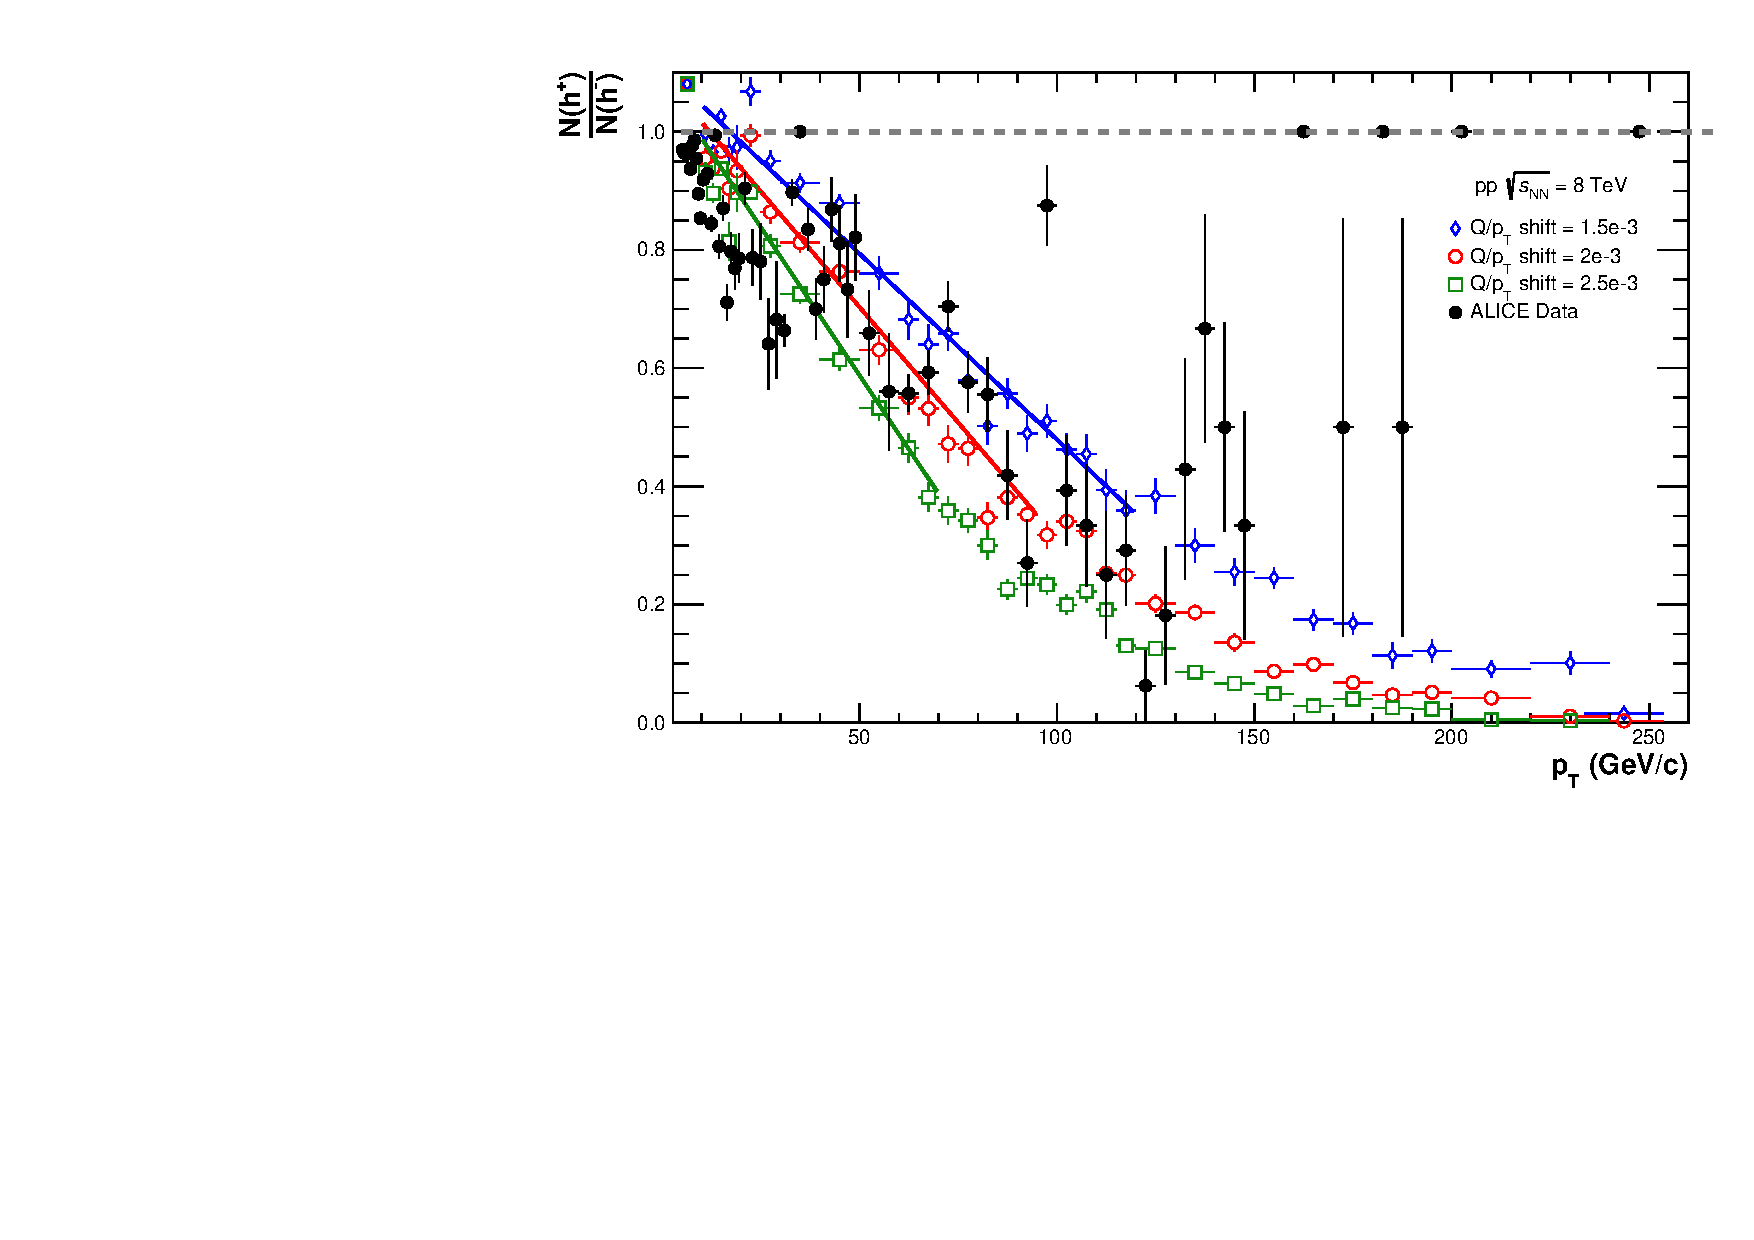
\includegraphics[width=15cm]{figures/QoverPtShift/QPTComparison.pdf}
    \caption{Comparison of different Q/\pT shift values.}
    \label{fig:QoverPtShift}
\end{figure}

Some additional uncertainties are required for \pPb. These are as follows:

\begin{itemize}
    \item Background fluctuations: In order to account for the uncertainty in the estimation of background fluctuations, a delta-\pT matrix formed by single-track embedding is used to smear the response instead of the random cones method that is used by default.
    \item Luminosity: As agreed with trigger coordination, the difference between expected (configured) downscaling factor and observed downscaling factor is propagated into the luminosity. Downscaling is a statistical process with finite precision, as events are rejected for downscaling randomly. In order to propagate the uncertainty on the luminosity into the spectrum, the raw spectrum is shifted by the corresponding uncertainty for EJ1 and EJ2 separately, and the unfolded spectrum for each is taken as a variation.
\end{itemize}

The components of the uncertainty are then added in quadrature. The different components of the systematic uncertainties for R = 0.2 jets are shown in Fig. \ref{fig:SystematicsSpectraR02} (for other jet radii and individual contributions, see appendix \ref{sec:AppendixSystematics}).

\begin{figure}
    \centering
    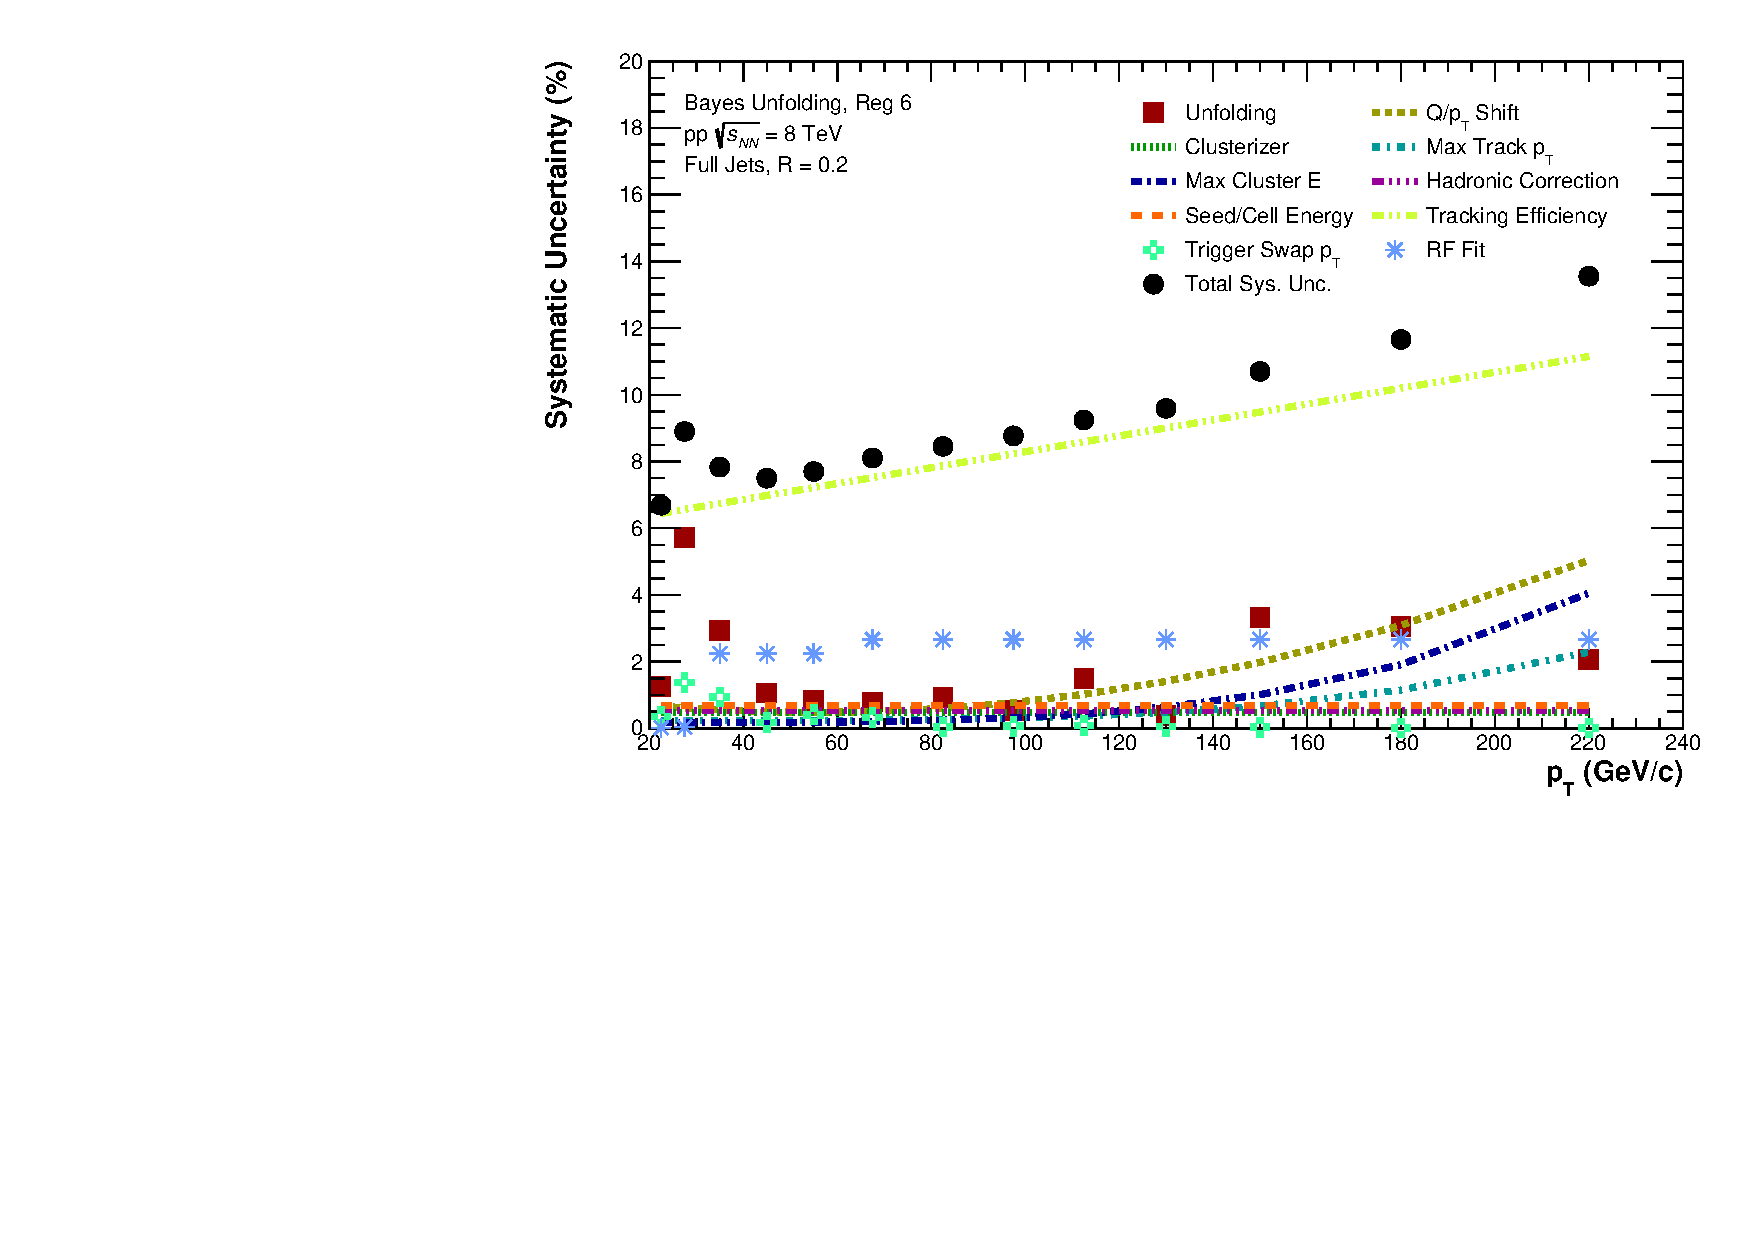
\includegraphics[width=15cm]{figures/Systematics/TotalSystematics_R02.pdf}
    \caption{All sources of systematic uncertainties, including the total systematic uncertainty with all components added in quadrature for \pp.}
    \label{fig:SystematicsSpectraR02}
\end{figure}

The equivalent plot for \pPb can be in in figure \ref{fig:SystematicsSpectraR02pPb}, and the equivalent appendix is \ref{sec:AppendixSystematicspPb}.

\begin{figure}
    \centering
    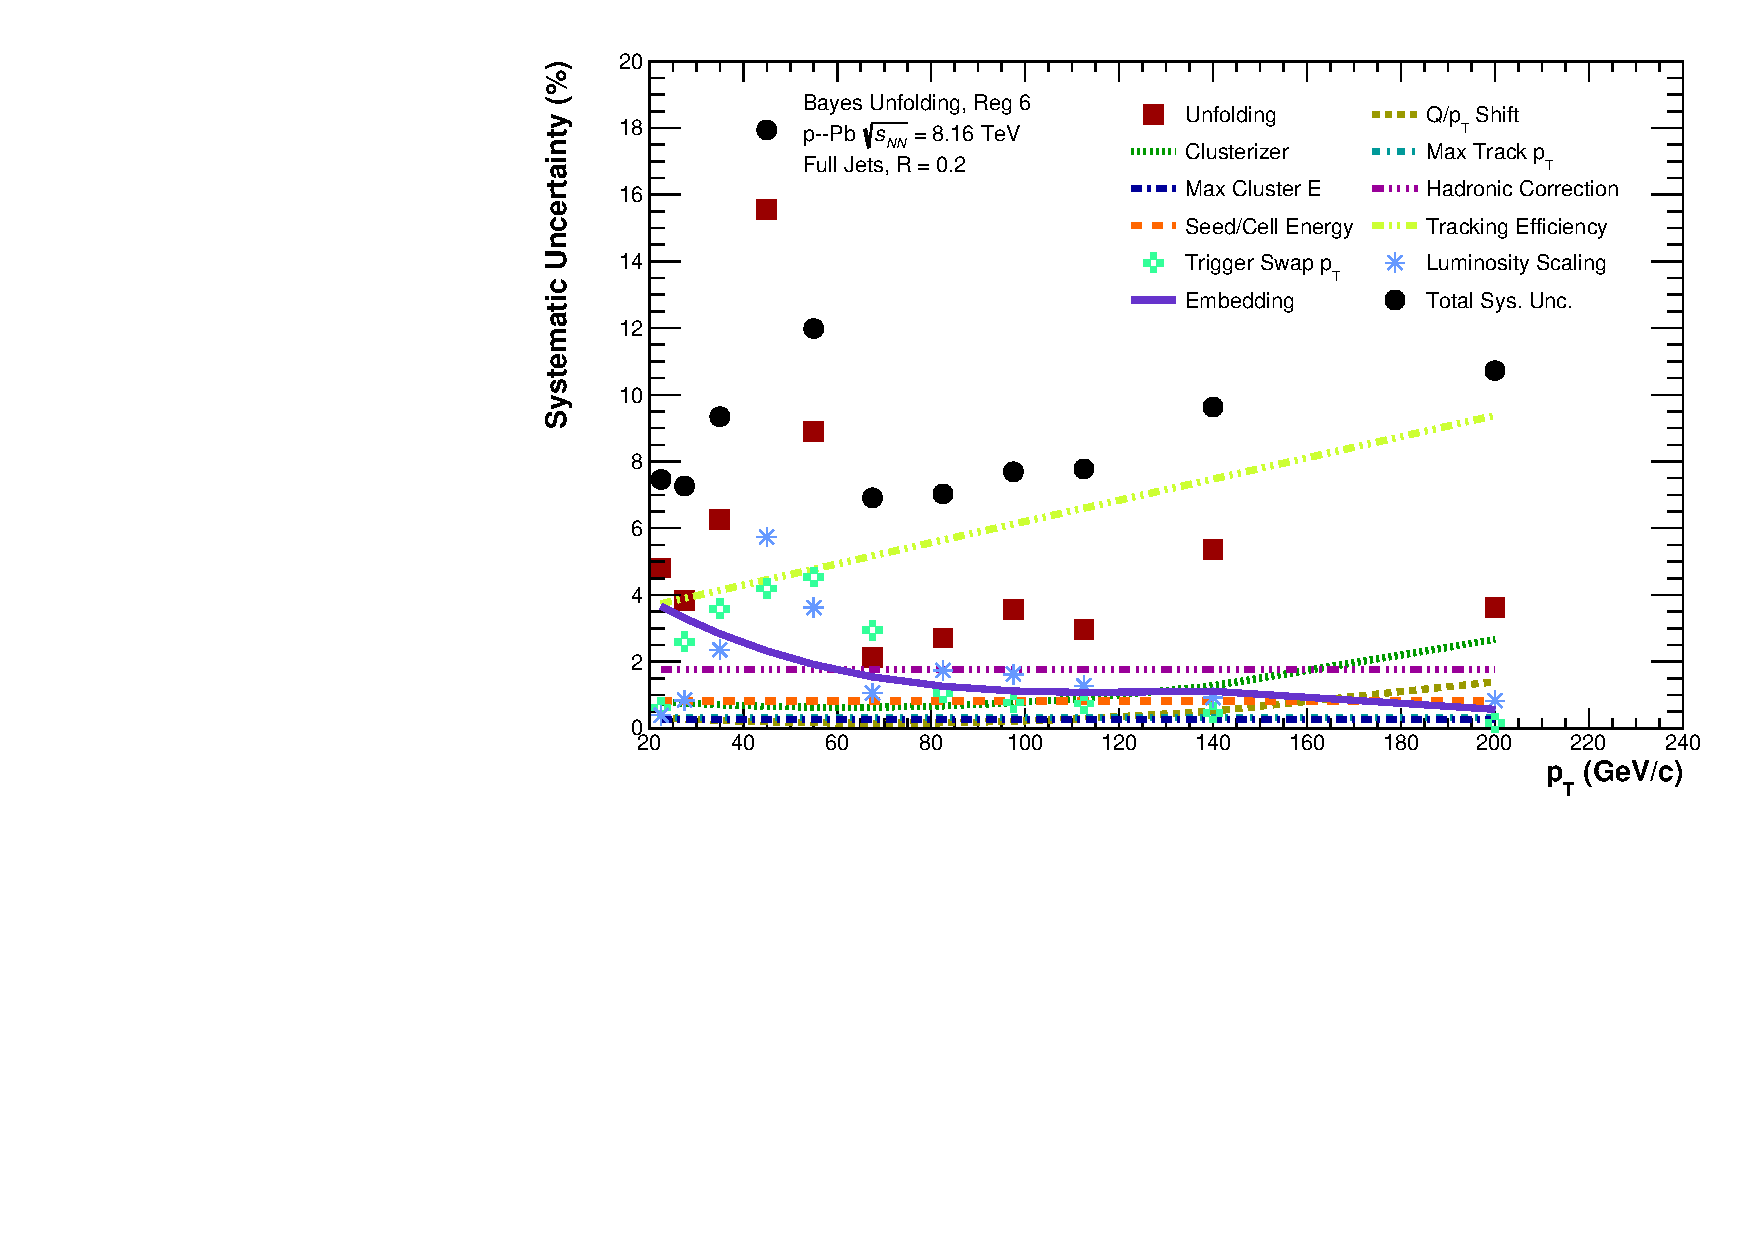
\includegraphics[width=15cm]{figures/pPbFigures/Systematics/TotalSystematics_R02.pdf}
    \caption{All sources of systematic uncertainties, including the total systematic uncertainty with all components added in quadrature for \pPb.}
    \label{fig:SystematicsSpectraR02pPb}
\end{figure}

\subsection{Cross-Section Ratios}
\label{sec:SystematicsRatios}

For the cross-section ratios, the same systematic contributions are considered. With the exception of the trigger rejection factor fit, trigger swap, and unfolding systematics, all contributions are calculated directly on the ratio, resulting in partial cancelling. The rejection factor fit is not included at all, since this contribution cancels entirely. The trigger swap and unfolding contributions for each cross-section in the ratio are added in quadrature to the total uncertainty. The different components of the systematic uncertainties for R = 0.2/0.3 jets are shown in Fig. \ref{fig:SystematicsRatiosR02} for \pp and \ref{fig:SystematicsRatiosR02pPb} for \pPb (for other jet radii and individual contributions, see appendix \ref{sec:AppendixSystematics} and \ref{sec:AppendixSystematicspPb}).

\begin{figure}
    \centering
    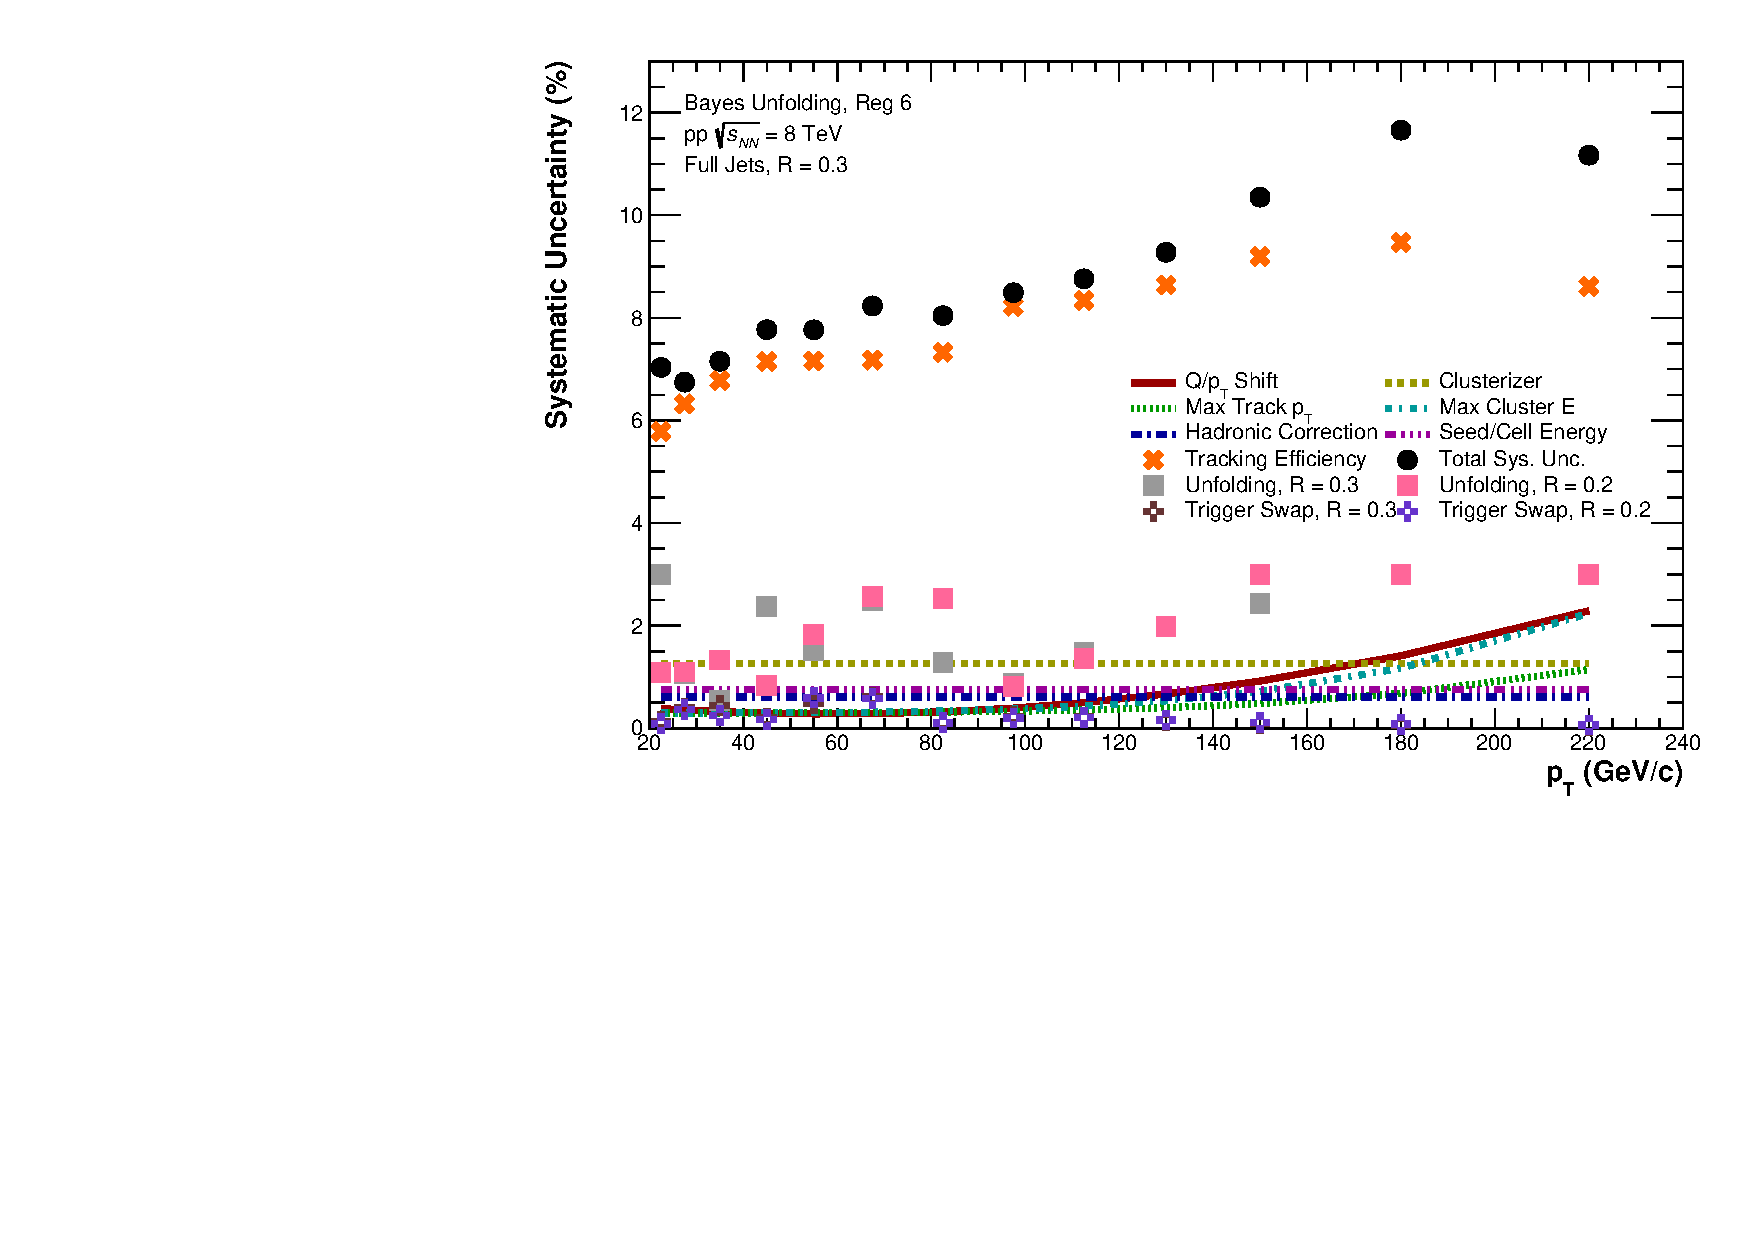
\includegraphics[width=15cm]{figures/Systematics/ratios/TotalSystematics_R02R03.pdf}
    \caption{All sources of systematic uncertainties, including the total systematic uncertainty with all components added in quadrature for \pp.}
    \label{fig:SystematicsRatiosR02}
\end{figure}

\begin{figure}
    \centering
    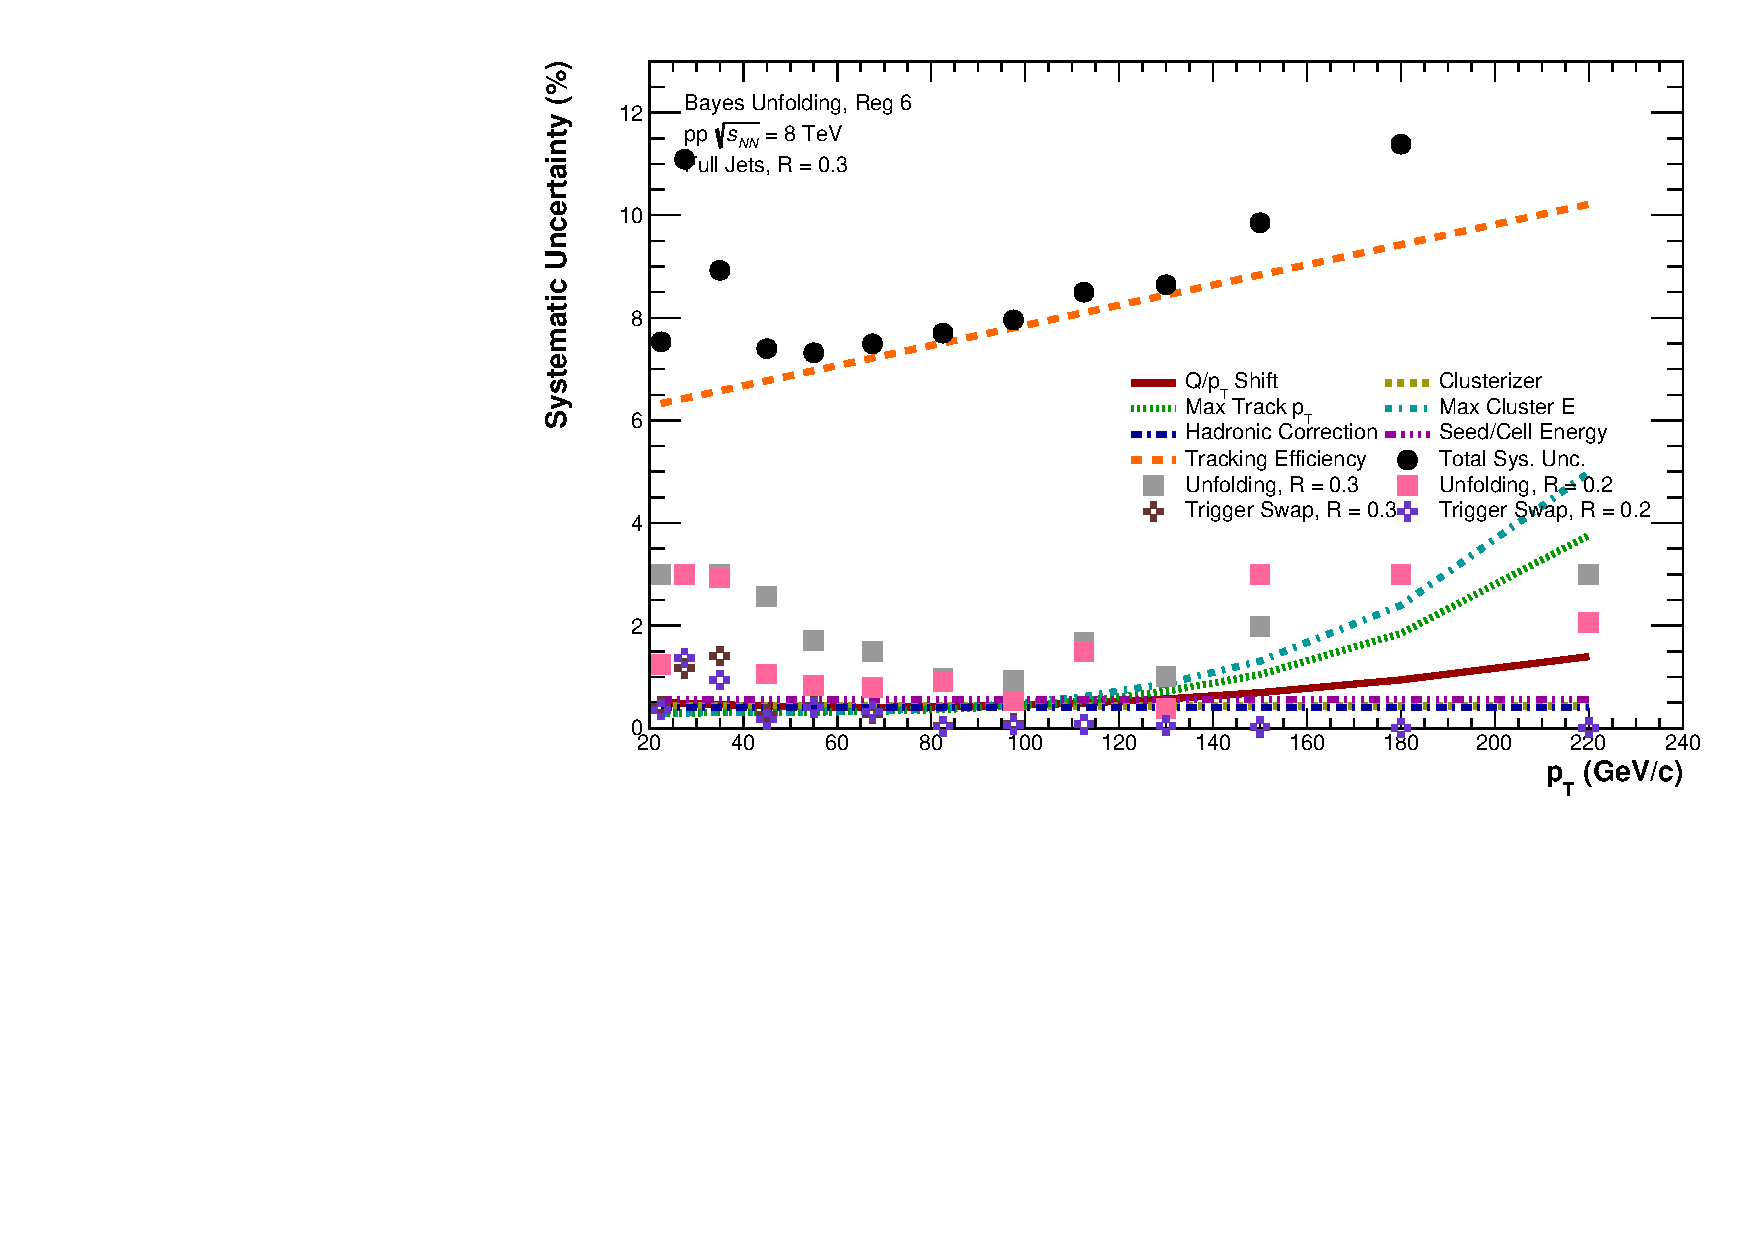
\includegraphics[width=15cm]{figures/pPbFigures/Systematics/ratios/TotalSystematics_R02R03.pdf}
    \caption{All sources of systematic uncertainties, including the total systematic uncertainty with all components added in quadrature for \pp.}
    \label{fig:SystematicsRatiosR02pPb}
\end{figure}

\subsection{Nuclear modification factor}
\label{sec:systematicsRpA}

For the nuclear modification factor, the same method is used that was used for the cross-section ratios. The trigger rejection factor fit will not cancel in this situation, and the same is true for the luminosity. The trigger swap and unfolding contributions for each cross-section in the ratio are added in quadrature to the total uncertainty. The background fluctuations uncertainty is also added in quadrature. The different components of the systematic uncertainties for R = 0.2 jets are shown in Fig. \textcolor{red}{Add RpPb systematics}. For other radii, see appendix \textcolor{red}{!!!} %\ref{sec:AppendixSystematicsRpPb}).